\documentclass[handout]{beamer} %[handout] pour supprimer la barre de navigation mais \pause ne fonctionne pas dans ce mode
\usepackage[frenchb]{babel}
\usepackage[T1]{fontenc}
\usepackage[utf8]{inputenc}


\usetheme{Frankfurt}

\title[Javabyrinthe]{Javabyrinthe \\ Projet d'Informatique Répartie}
\author{Alexandre Brehmer \and Christophe Cluizel  \and Anthony Courtin \and Céline Leduc \and Charlotte Touchard \and Simon Wallon}
\institute{INSA Rouen}
\date{12 mai 2015}

%ajoute la numérotation des pages et nombre pages total
\addtobeamertemplate{footline}{\hfill\insertframenumber/\inserttotalframenumber\hspace{2em}\null}

%indiquer le chemin du dossier des images
\graphicspath{{}{image/}}

\usepackage{array}
\usepackage{url}
\usepackage{hyperref}


\begin{document}
  \begin{frame}[plain]
  \titlepage
  \end{frame}

  \AtBeginSection[]
  {
    \begin{frame}
    \frametitle{Sommaire}
    \tableofcontents[currentsection, hideothersubsections]

    \end{frame}
  }

  % ============== Introduction ================
\chapter{Introduction}

% ----------- Contexte du projet -----------
\section{Contexte du projet}
\TODO{Céline}

% On est en ASI4, on a cours d'info Rep et on doit faire un projet blablabla…

% ----------- Principe général -----------
\section{Principe général}
\TODO{Céline}

% On va faire un super projet de la mort trop cool sur un labyrinthe multijoueur blablabla…

% ----------- Principales technologies utilisées -----------
\section{Principales technologies utilisées}
\TODO{Charlotte}

% Ce que l'on a dit pdt la réunion, java, socket…
% pourquoi c'est techno
% avantage/inconvénient

  % ========== Choix techniques ===========
\section{Choix techniques}

  \subsection{Logique métier}
    \begin{frame}
      \frametitle{Choix techniques}
      \begin{itemize}
        \item Langage de programmation: \textbf{Java} \vspace{1cm}
        \item Communication client-serveur: \textbf{RMI}
        \begin{itemize}
          \item Orienté objet
          \item Gestion des exceptions
        \end{itemize}
      \end{itemize}
    \end{frame}

  \subsection{Graphisme}
    \begin{frame}
      \frametitle{Choix techniques}
      \begin{itemize}
        \item Interface graphique: \textbf{Slick2D}
      \end{itemize}
      \begin{center}
        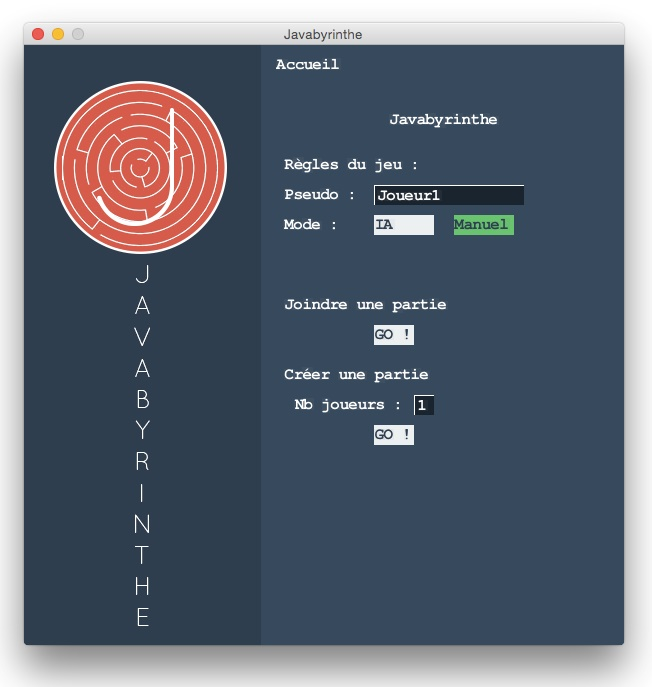
\includegraphics[scale=0.4]{image/menuJavabyrinthe.jpg}
      \end{center}
    \end{frame}

  \TODO{Christophe, Simon, Charlotte}

  % ========== Démonstration ===========
\section{Démonstration}

    \begin{frame}
        \frametitle{Démonstration}


    \end{frame}

  % ========== Analyse critique ===========
\section{Analyse critique}

	\begin{frame}
		\frametitle{Analyse critique}

		\begin{itemize}
		\item \textbf{Points forts}
			\begin{itemize}
				\item Possibilité de jouer à quatre sur une partie
				\item Générateur automatique de labyrinthes de taille personnalisée
				\item L'utilisateur n'a pas besoin de compiler son code
			\end{itemize}
		\vspace{10px}
		\item \textbf{Pas de problèmes non-résolus}
		\vspace{10px}
		\item \textbf{Améliorations possibles}
			\begin{itemize}
				\item Exécution de l'IA sur le serveur
				\item Extension à différents langages
				\item Code de l'IA directement dans l'interface graphique
			\end{itemize}
		\end{itemize}
	\end{frame}

  % ========== Conclusion ===========
\section{Conclusion}

  \begin{frame}
    \frametitle{Conclusion}

  \end{frame}


\end{document}
